% --- CÓDIGO ATUALIZADO para Analise/bubble_sort_analise.tex ---

\subsubsection*{Análise de Complexidade e Teste de Mesa - Bubble Sort}

\qquad Esta seção apresenta o teste de mesa do \textit{Bubble Sort} e a derivação de sua função de tempo $T(n)$.

\paragraph{Teste de Mesa}
\qquad A Figura \ref{fig:bubble_mesa} mostra a execução do \textit{Bubble Sort}, acompanhando os valores das variáveis \texttt{i} e \texttt{j} e o estado do vetor a cada comparação e troca. É possível observar o maior elemento sendo deslocado para o final do vetor a cada passagem do laço externo.

% --- IMAGEM DO TESTE DE MESA ---
\begin{figure}[htbp]
    \centering
    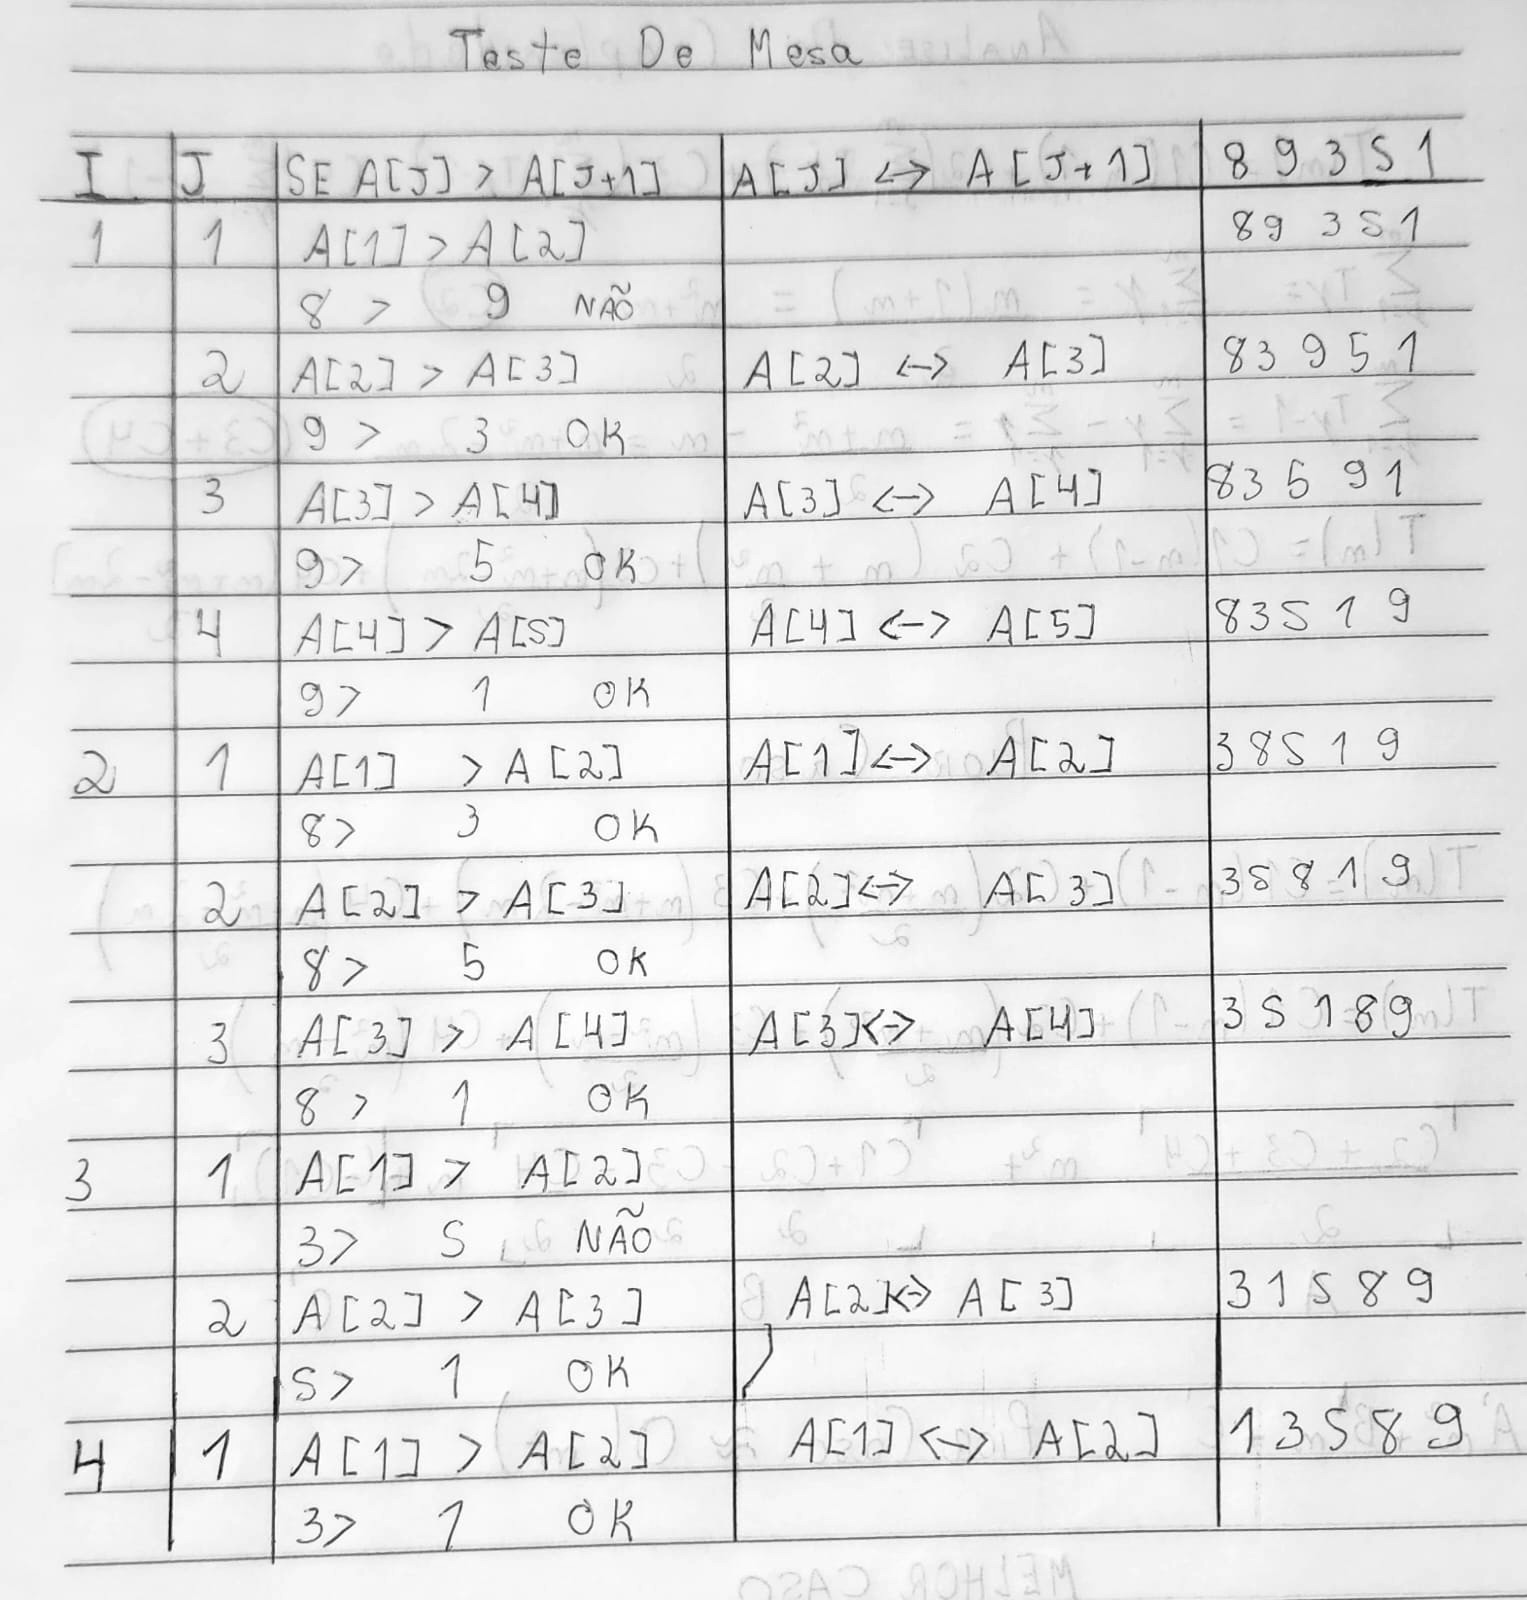
\includegraphics[width=1.0\textwidth]{Imagens/Bubble Sort/testedemesa-bubble.jpg}
    \caption{Teste de Mesa do algoritmo Bubble Sort (elaborado pelo autor).}
    \label{fig:bubble_mesa}
\end{figure}

\paragraph{Análise Matemática Geral}
\qquad A Figura \ref{fig:bubble_analise_geral} apresenta a dedução da função de tempo $T(n)$ a partir da tabela de custos e da frequência de execução dos laços aninhados.

% --- IMAGEM DA ANÁLISE DE COMPLEXIDADE GERAL ---
\begin{figure}[htbp]
    \centering
    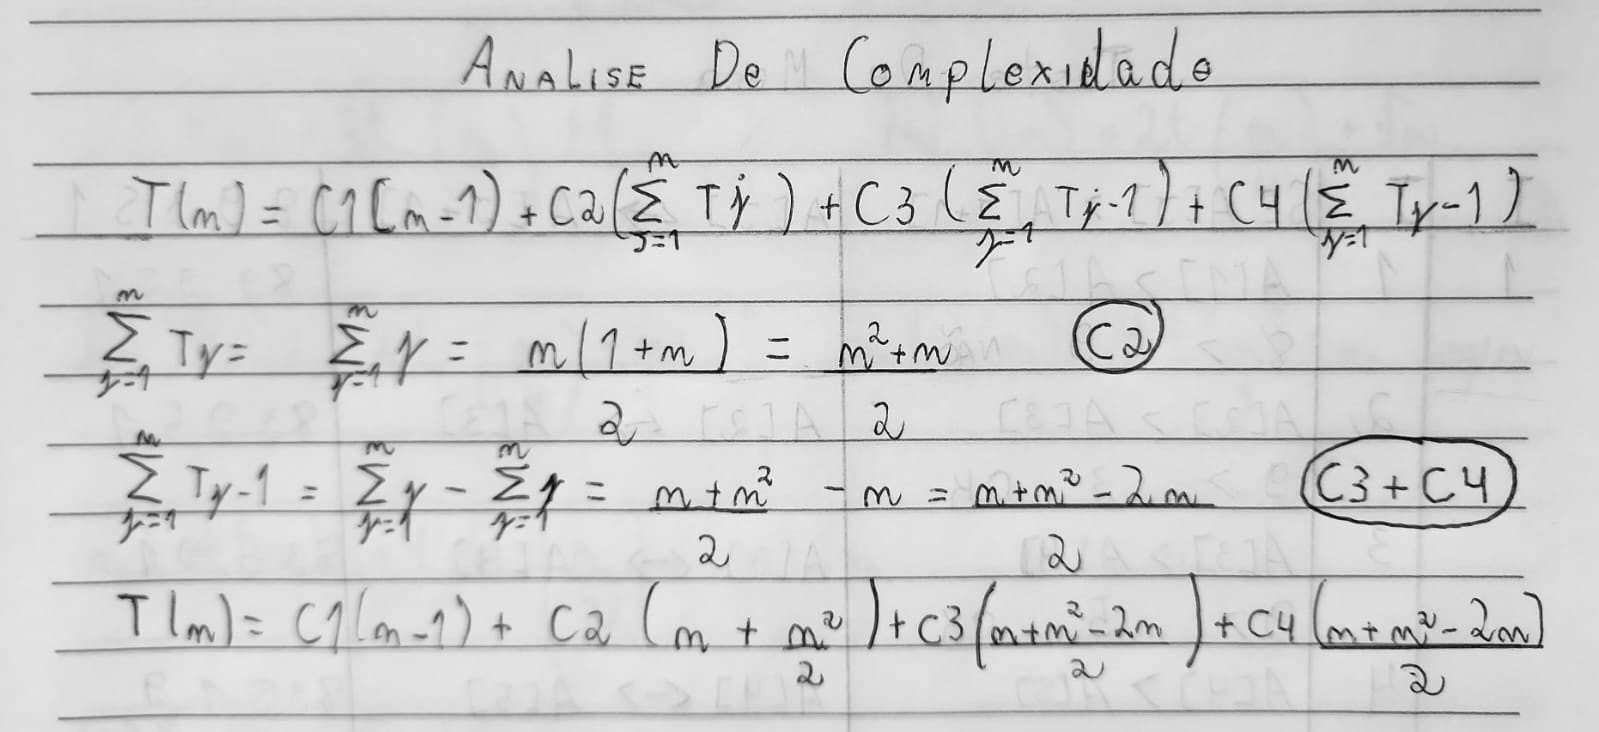
\includegraphics[width=1.0\textwidth]{Imagens/Bubble Sort/analisedecomplexidade-bubble.jpg}
    \caption{Análise de Complexidade geral do Bubble Sort (elaborado pelo autor).}
    \label{fig:bubble_analise_geral}
\end{figure}


\paragraph{Análise por Cenário}
\qquad A seguir, a função de tempo é analisada separadamente para os três cenários: melhor, pior e médio caso.

\qquad No \textbf{melhor caso} (Figura \ref{fig:bubble_melhor_math}), mesmo sem a necessidade de trocas, a implementação ainda percorre os laços por completo, o que mantém a complexidade em $O(n^2)$.

% --- IMAGEM DO MELHOR CASO ---
\begin{figure}[htbp]
    \centering
    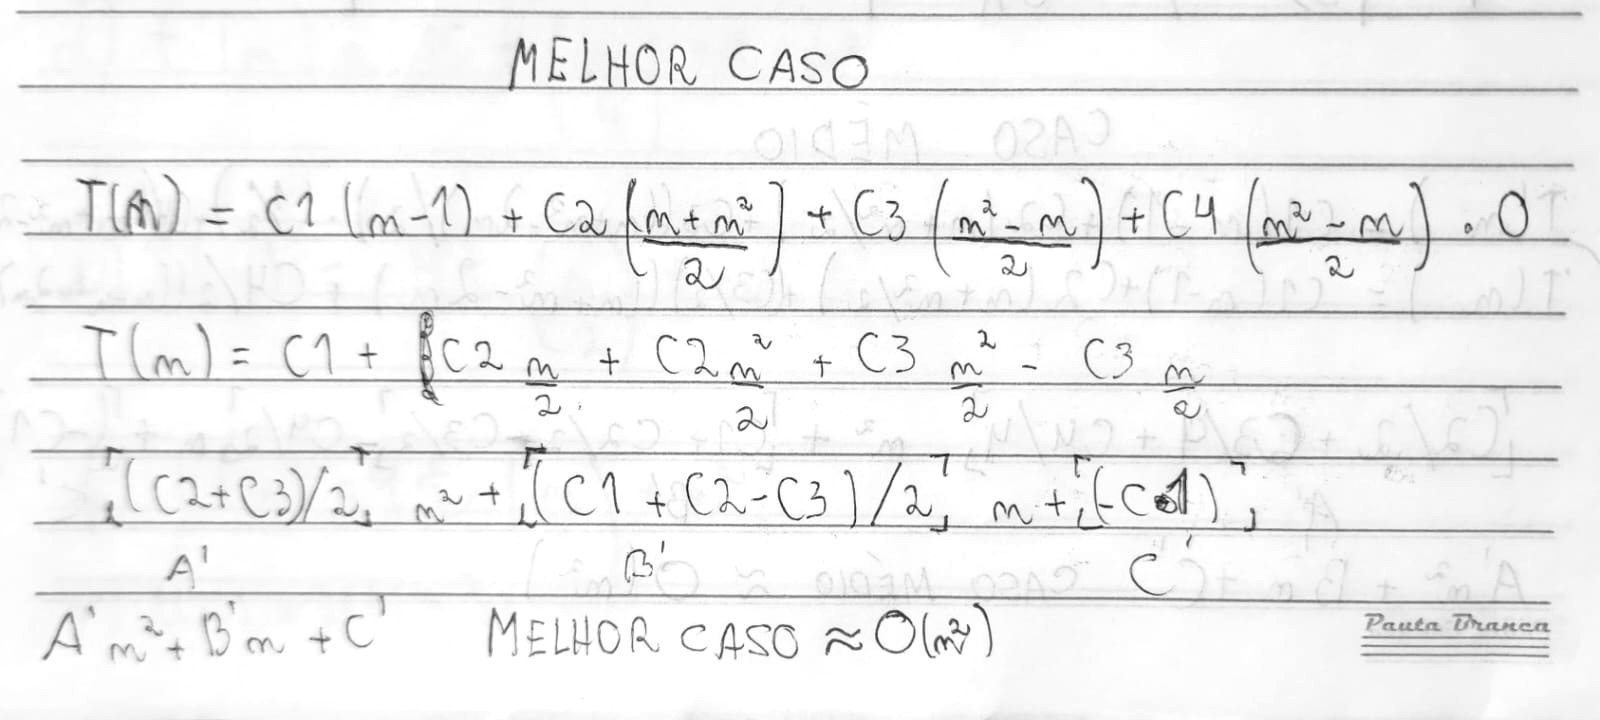
\includegraphics[width=0.9\textwidth]{Imagens/Bubble Sort/melhorcaso-bubble.jpg}
    \caption{Desenvolvimento matemático para o Melhor Caso do Bubble Sort (elaborado pelo autor).}
    \label{fig:bubble_melhor_math}
\end{figure}

\qquad No \textbf{pior caso} (Figura \ref{fig:bubble_pior_math}), com o vetor em ordem inversa, ocorre o número máximo de trocas, o que também resulta em $O(n^2)$.

% --- IMAGEM DO PIOR CASO ---
\begin{figure}[htbp]
    \centering
    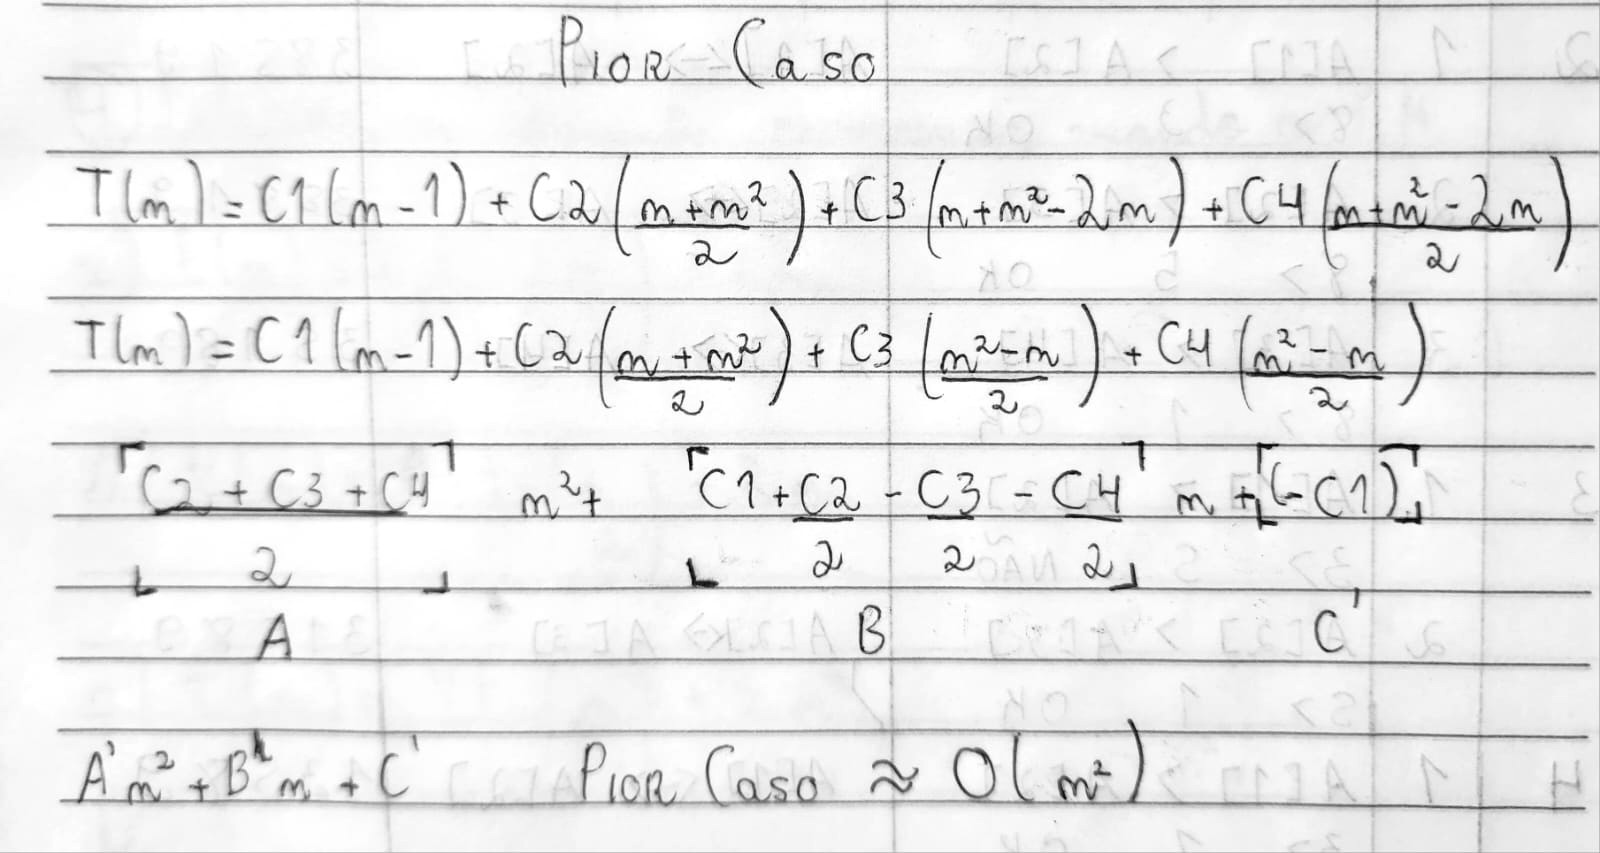
\includegraphics[width=0.9\textwidth]{Imagens/Bubble Sort/piorcaso-bubble.jpg}
    \caption{Desenvolvimento matemático para o Pior Caso do Bubble Sort (elaborado pelo autor).}
    \label{fig:bubble_pior_math}
\end{figure}

\qquad No \textbf{caso médio} (Figura \ref{fig:bubble_medio_math}), o número de comparações continua sendo o fator dominante, o que resulta na mesma complexidade $O(n^2)$.

% --- IMAGEM DO CASO MÉDIO ---
\begin{figure}[htbp]
    \centering
    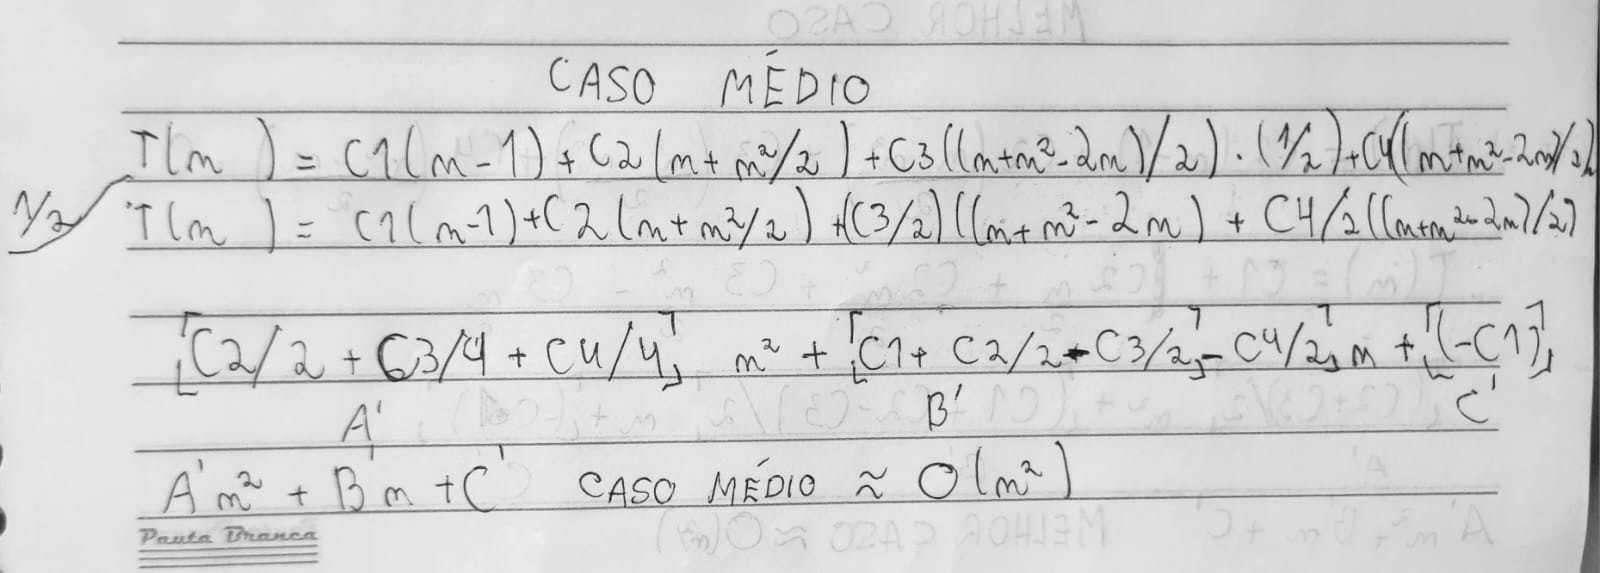
\includegraphics[width=0.9\textwidth]{Imagens/Bubble Sort/mediocaso-bubble.jpg}
    \caption{Análise da função de tempo para o Caso Médio do Bubble Sort (elaborado pelo autor).}
    \label{fig:bubble_medio_math}
\end{figure}

\FloatBarrier

\qquad Quanto à \textbf{complexidade de espaço}, o \textit{Bubble Sort} apresenta complexidade $O(1)$, já que a ordenação é feita \textit{in-place}, sem uso de estruturas auxiliares proporcionais a $n$.